\documentclass[11pt]{article}
%%
%% Package includes to provide the basic style
%%
\usepackage[top=3.5cm, bottom=3.5cm, left=2.5cm, right=2.5cm]{geometry}
\usepackage{hyperref}
\usepackage{pdfpages}
\usepackage{algorithm2e}
\usepackage[authoryear]{natbib}
\bibliographystyle{plainnat}
\usepackage{appendix}
\usepackage{pgfplotstable}
\usepackage[font={color=darkgray,footnotesize, sf, it}]{caption}
\usepackage{amsmath}
\usepackage{helvet}
\usepackage{wrapfig}
\usepackage{multicol}
\usepackage[eulergreek]{sansmath}
\usepackage{listings}
\usepackage{setspace}
\usepackage{graphicx}
\usepackage{longtable}
\usepackage{minted}
\usepackage{relsize}
\linespread{1.2}
\lstset { %
    language=C++,
    backgroundcolor=\color{black!5}, % set backgroundcolor
    basicstyle=\ttfamily\footnotesize,% basic font setting
}
\usepackage{bchart}
\usepackage{booktabs}
\usepackage{xcolor}

\definecolor{skyblue}{RGB}{203,240,255}
\definecolor{forestgreen}{RGB}{0,96,50}
\definecolor{indigo}{RGB}{4,87,239}
\definecolor{darkindigo}{RGB}{1,40,112}
\definecolor{darkpurple}{RGB}{32,14,104}
\definecolor{apple}{RGB}{0,158,13}
\definecolor{bad}{RGB}{239,55,55}
\definecolor{badtoavg}{RGB}{247,128,98}
\definecolor{avg}{RGB}{255,218,117}
\definecolor{avgtogood}{RGB}{190,247,140}
\definecolor{good}{RGB}{102,226,102}

\setlength{\parindent}{0em}
\setlength{\parskip}{1em}
\setlength\parindent{0pt}

\usepackage{titling}
\usepackage{titlesec}
\pretitle{\Huge\bfseries}
\posttitle{\par}

\titlespacing\section{0pt}{12pt plus 4pt minus 2pt}{0pt plus 2pt minus 2pt}
\titlespacing\subsection{0pt}{12pt plus 4pt minus 2pt}{0pt plus 2pt minus 2pt}
\titlespacing\subsubsection{0pt}{12pt plus 4pt minus 2pt}{0pt plus 2pt minus 2pt}

\usepackage[english]{babel}
\usepackage[utf8]{inputenc}
\usepackage{fancyhdr}
 
\pagestyle{fancy}
\fancyhf{}
\rhead{cjd47}
\lhead{CM30141: \textit{Theory of Human-Computer Interaction}}
\cfoot{\thepage} 
\renewcommand{\headrulewidth}{1pt}
\renewcommand{\footrulewidth}{1pt}

\newcommand\wordcount[1]{
\vfill
\textit{Word count: {#1} words (not inc. Citations, Figures or References)}}

\newcommand\essaytitle[1]{
\begin{LARGE}
\textbf{{#1}} \\
\end{LARGE}}

\newcommand\sectiontitle[1]{
\begin{large}
\textbf{{#1}} \medskip \\ 
\end{large}}

%%
%% END OF DEFINITIONS
%%

\begin{document}
\essaytitle{Critical Review: Exploring Interactions with Physically Dynamic Bar Charts}

\sectiontitle{Introduction}
Studies investigating how data can be effectively presented to, explored and interpreted by users forms the core part of Information Visualisation (`InfoVis') to support users in the decision-making process. This review summarises and critically analyses \citet{taher2015} whose paper explores the use of physically dynamic bar chart as a device for exploring user interactions with visualisations of data, to determine future work in this domain of Information Visualisation.

\sectiontitle{Summary of Contributions}
\citeauthor{taher2015} seeks to extend existing work on use of physical visualisations (\textit{physicalizations}) to investigate how users interact with \textit{physically dynamic} bar charts as a way of exploring and manipulating shape-changing datasets in the physical world. Much of the existing work reliant on use of physicalizations involve problematic \textit{static} models that do not respond to user interactions \citep{jansen2013} and are therefore ``\textit{disconnected}'' from the source of the data when they are created. With the advent of shape-changing technology and tangible interfaces \citep{rasmussen2012}, there is a window of opportunity for the manufacture of physically dynamic displays to help decision makers reason about and manipulate data sets in a non-virtual and non-static way. It is this motivation that leads \citeauthor{taher2015} to explore the ways users interact with data displayed in this mode to understand whether physical interactions (such as touching specific data points) or gestures (such as swiping a touch-screen) or a combination of the two is more intuitive to users interacting with data visualisations in order to solve common problems.

The point system described by the article is \textit{EMERGE} - a $10\times10$ set of dynamic self-actuating rods with an RGB display projected onto it (Figure \ref{fig:taher2015-emerge}). This system allows users to interact with the dataset it represents using a subset of 4 task-sets derived from sub-categories of the taxonomy of interactive dynamics for visual analysis described by \citet{heer2012} - \textit{annotation}, \textit{filtering}, \textit{organisation} and \textit{navigation} (Table \ref{tbl:taher2015-user-study}).

\begin{figure}[H]
\centering
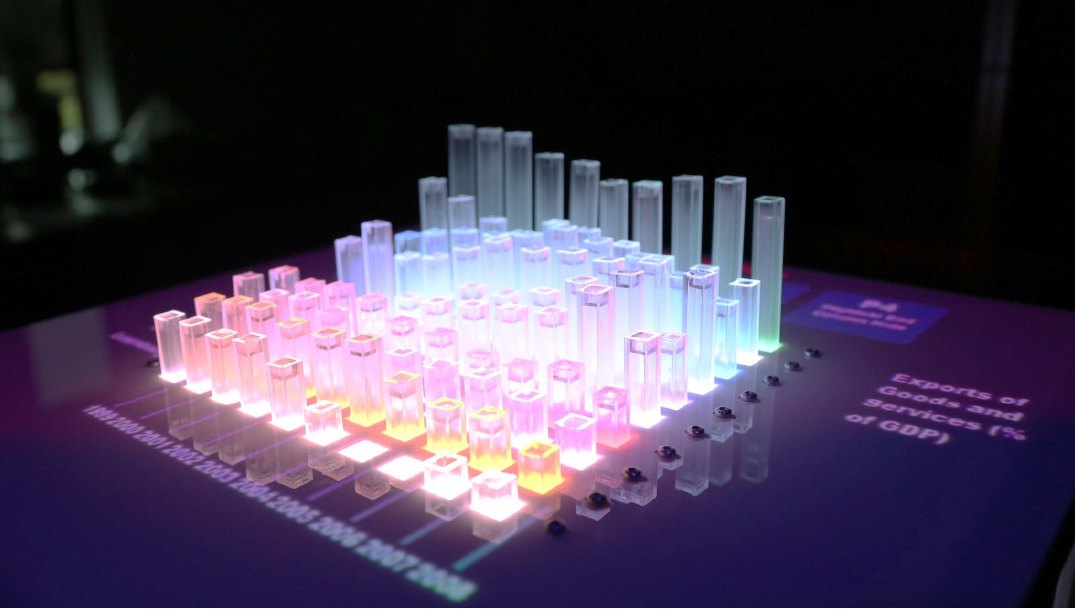
\includegraphics[width=0.5\textwidth]{img/taher2015-emerge.png} 
\caption{EMERGE: Exploring Interactions with Physically Dynamic Bar Charts using actuating physical rods and RGB LEDs to display international export data.}\label{fig:taher2015-emerge}
\end{figure}

\begin{table}[H]
\centering
\caption{Task-sets and interaction techniques explored during the user study: \textit{annotation}, \textit{filtering}, \textit{organisation} and \textit{navigation} with the }\label{tbl:taher2015-user-study}
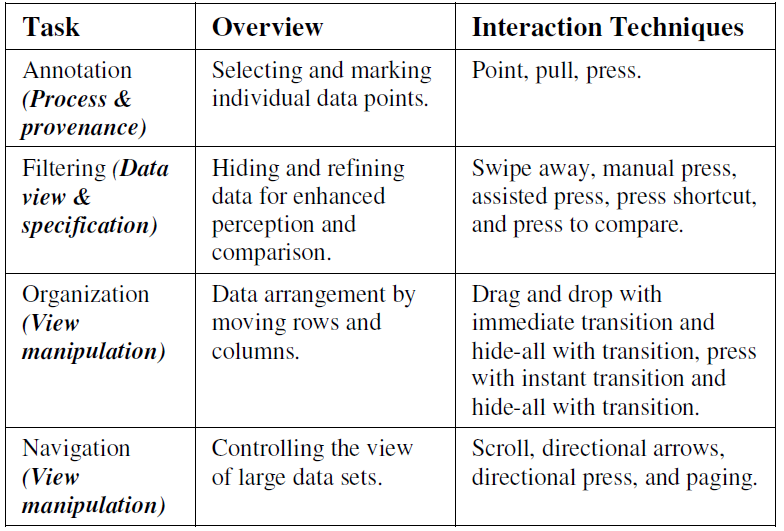
\includegraphics[width=0.65\textwidth]{img/taher2015-user-study.png} 
\end{table}

\citeauthor{heer2012} lay out 3 categories in their model - \textit{Data and View Specification},
\textit{View Manipulation}, and \textit{Process and Provenance}. (Figure \ref{fig:heer2012-taxonomy}). In this sense, the choice of subcategories by \citeauthor{taher2015} is somewhat arbitrary and limited in their scope, but invites further research into different forms of interactions with physicalisations.

\begin{figure}[H]
\centering
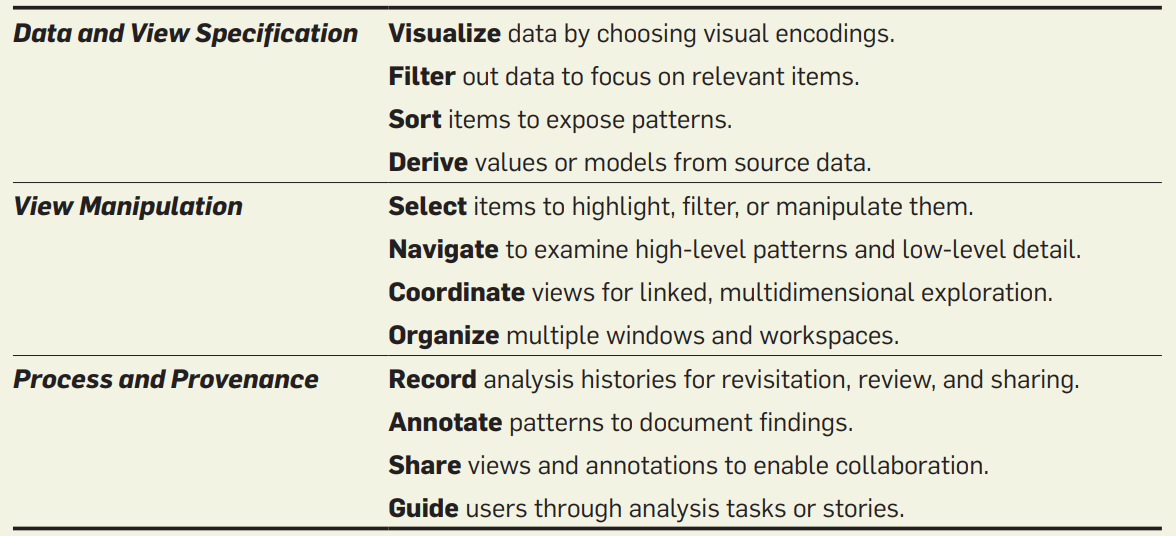
\includegraphics[width=0.7\textwidth]{img/heer2012-taxonomy.png} 
\caption{EMERGE: Exploring Interactions with Physically Dynamic Bar Charts using actuating physical rods and RGB LEDs to display international export data.}\label{fig:heer2012-taxonomy}
\end{figure}

The main contributions of \citet{taher2015} is threefold. First, the authors present a set of 14 potential interactions 


\sectiontitle{Justifications for Conclusions}
...

\begin{figure}[H]
\minipage{0.5\textwidth}
\centering
  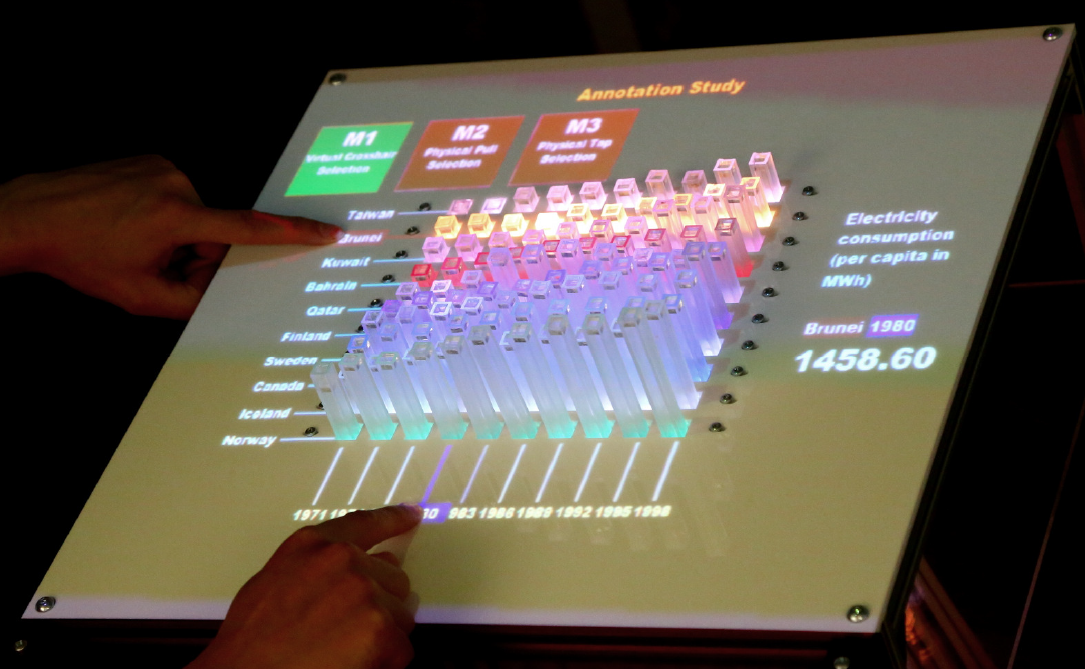
\includegraphics[height=3.5cm]{img/taher2015-annotation.png}
  \caption{Annotation (Point technique).}\label{fig:taher2015-annotation}
\endminipage\hfill
\minipage{0.5\textwidth}%
\centering
  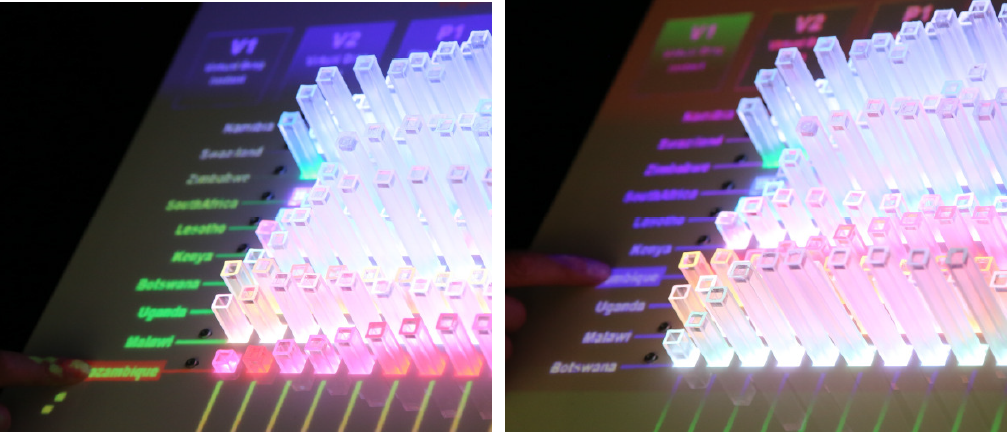
\includegraphics[height=3.5cm]{img/taher2015-organize.png}
  \caption{Organisation (Drag and Drop technique).}\label{fig:taher2015-organize}
\endminipage
\end{figure}

\begin{figure}[H]
\centering
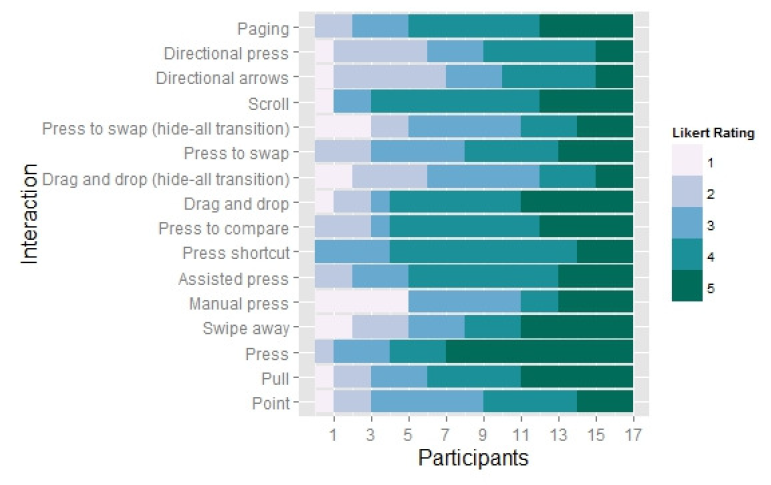
\includegraphics[width=0.5\textwidth]{img/taher2015-likert.png} 
\caption{Likert scale ratings for helpfulness of interaction
techniques. Range = 1: Strongly Disagree, 5: Strongly Agree.}\label{fig:taher2015-likert}
\end{figure}

\sectiontitle{Limitations and Suggested Further Work}
...

\sectiontitle{Conclusion}
...

\wordcount{0}

\newpage
\small
\bibliography{bib2}
\normalsize
\end{document}